% Template for PLoS
% Version 1.0 January 2009
%
% To compile to pdf, run:
% latex plos.template
% bibtex plos.template
% latex plos.template
% latex plos.template
% dvipdf plos.template

% \documentclass[10pt, twocolumn]{article}
\documentclass[10pt]{article}
\usepackage{amsmath}
\usepackage{amssymb}
\usepackage{graphicx}
\usepackage{color} % for revision purposes only, may be not present in the final file
% cite package, to clean up citations in the main text. Do not remove.
\usepackage{cite}
\usepackage{color}
\usepackage{indentfirst} %% LM: in order to indent the first paragraph of each section
\usepackage{url} %% LM: in order to include nice urls
\usepackage{booktabs} %% LM: nice tables...
\usepackage{subfigure} % LM: panels
\usepackage{xr} % automatic cross-referencing
\externaldocument{Text_S2}
% Use doublespacing - comment out for single spacing
%\usepackage{setspace}
%\doublespacing

\topmargin 0.0cm
\oddsidemargin 0.5cm
\evensidemargin 0.5cm
\textwidth 16cm
\textheight 21cm

\usepackage[labelfont=bf,labelsep=period,justification=raggedright]{caption}

\bibliographystyle{plos2009}% 

\makeatletter
\renewcommand{\@biblabel}[1]{\quad#1.}
\makeatother


% Leave date blank
\date{}

\pagestyle{myheadings}
%% ** EDIT HERE **


%% ** EDIT HERE **
%% PLEASE INCLUDE ALL MACROS BELOW

%% END MACROS SECTION

\begin{document}

% Title must be 150 characters or less
\begin{flushleft}
{\Large
\textbf{Spatiotemporal Dynamics of Foot-and-Mouth Disease Virus in South America}
}
% Insert Author names, affiliations and corresponding author email.
\\
Luiz Max Carvalho$^{1,2\ast}$,
Guy Baele$^{3}$,
Nuno Rodrigues Faria$^{3,4}$,
Andres M.~Perez$^{5}$,
Marc A.~Suchard$^{6,7}$
Philippe Lemey$^{3}$,
Waldemir de Castro Silveira$^{1}$
\\
\bf{1} Pan American Center for Foot-and-Mouth Disease (PAHO/WHO), Duque de Caxias, Rio de Janeiro, Brazil.
\\
\bf{2} Program for Scientific Computing (PROCC), Oswaldo Cruz Foundation, Rio de Janeiro, Rio de Janeiro, Brazil.
\\
\bf{3} Department of Microbiology and Immunology, Rega Institute -- KU Leuven, Leuven, Belgium.
\\
\bf{4} Department of Zoology, University of Oxford, Oxford, United Kingdom.
\\
\bf{5} Department of Veterinary Population Medicine, University of Minnesota, St. Paul, United States of America.
\\
\bf{6} Departments of Biomathematics and Human Genetics, David Geffen School of Medicine at UCLA, University of California, Los Angeles,  United States of America.\\
\bf{7} Department of Biostatistics, UCLA Fielding School of Public Health, University of California, Los Angeles,  United States of America.
\\
$\ast$ E-mail: lmax.procc@gmail.com
\end{flushleft}
% Please keep the abstract between 250 and 300 words
\section*{Abstract}

%GB: is 'free' the term we want to be using here? %LM: Yes.
Although foot-and-mouth disease virus (FMDV) occurrence has diminished over the years, the virus still circulates in certain areas of South America and the risk of re-emergence in previously free areas is a constant threat.
While the molecular epidemiology of FMDV in South America has been subject of several studies recently, an integrated quantitative approach to incorporate environmental and epidemiological data into the analyses is still lacking.
In this study, we apply state-of-the-art Bayesian phylogeography to the most comprehensive data sets of VP1 (1D) sequences from FMDV serotypes A and O collected in South America to date and analyse the temporal and spatial variation of FMDV and test evolutionary hypotheses.

We found that South American FMDV serotypes A and O exhibit rate variation among lineages and are best fitted by different relaxed molecular clock models (A: log-normal; O: exponential).
The phylogeographic analysis showed significant viral flow between Venezuela, Colombia and Ecuador while Brazil, Uruguay and Argentina also formed a well-connected sub network.
Using data on livestock (cattle, sheep and pigs) trade and geographic distance also allowed us to assess the importance of each of these predictors in viral flow, showing geographic distance to be the best predictor of serotype A spatial spread while the trade of live cattle was the strongest predictor of serotype O spread on the continent.

Key-words: Phylogeography, foot-and-mouth disease virus, South America, animal trade, BEAST.

\section*{Author Summary} % 150--200 words
Foot-and-mouth diseases virus (FMDV) 
is a rapidly evolving and highly infectious livestock pathogen.
In South America, although some molecular epidemiology studies are available, little is known about the virus phylodynamics.
In this paper we analyse all available VP1 sequences of FMDV serotypes A and O isolated in South America to unravel the spatial and temporal dynamics of the virus on the continent.
We show both serotypes present temporal structure and then estimate times to most recent common ancestor of $\approx 70$ and $\approx 20$ years for serotypes A and O, respectively. 
However, spatially, serotype O presents a dispersal rate four times faster than serotype A.
Additionally, we found that Brazil is a hub for serotype A spread but not for serotype O, while Colombia and Ecuador seem to be more important for serotype O dispersal on the continent.
We identified the trade of live cattle as the most important predictor of serotype O, while for serotype A geographic distances seem to best predict viral flow between South American countries.
Taken together, these results show that FMDV serotypes' different biology reflects in their different spatial dispersal patterns and reinforces the view that the trade of live cattle, specially across national borders (short range migration) is an important threat to control programmes.   

\section*{Introduction}

Foot-and-mouth disease virus (FMDV) is a rapidly evolving picornavirus and the causative agent of foot-and-mouth disease (FMD), the most important disease of domestic and wild cloven-hoofed animals~\cite{review}.
Three of the seven FMDV serotypes (A, O, and C) circulate in certain areas of South America.
Serotype A has been responsible for epidemics that are typically larger and more extensive than those caused by other serotypes and that, in recent years, have been limited to the 
Southern cone of the continent~\cite{Perez2001, Malirat2012}.
Although serotype O has historically been the most prevalent serotype on the continent, in recent years it has been limited to areas in the Andean region~\cite{andean}.
Identification of serotype C in recent decades was limited to one case in the Brazilian Amazon.
Historical reports suggest that FMDV introduction in South America, in the late years of the 19th century, is  related to European colonization~\cite{tully}. 
By the 1970's, FMD was widespread in South America, with occurrence of multiple subtypes in large-scale epidemics~\cite{Saraiva2003}.

In South America, FMD control and eradication has traditionally been pursued using a combination of mass vaccination programs~\cite{vaccinationSA} and control of animal movements from areas in which FMDV infection was suspected.
Over time, passive and active surveillance programs have, with heterogeneous success, succeeded to early detect FMDV.
Phylogenetic analyses have already proved useful in veterinary public health both by recovering the transmission pathways from genetic data~\cite{cottam2007, cottam2008} and providing insight into the processes that drive re-emergence~\cite{combining}.

More recently, molecular epidemiology tools have been utilized to infer the origin and evolutionary history of emerging strains~\cite{Perez2001, Malirat2007, andean, Malirat2011, Maradei2013}.
However, as pointed out by Di Nardo, Knowles \& Paton (2011)~\cite{combining}, a joint evaluation of epidemiological, environmental and genetic data has usually been performed outside of an unified quantitative framework.
In this context, Bayesian phylogeography offers a statistical framework to combine multiple sources of information in order to understand the spatio-temporal dynamics of FMDV and perform evolutionary hypothesis testing.

Another important research goal is to gain insight into the main determinants of viral spread in the continent.
Animal movements constitute a major threat to eradication programmes, being an important driving factor for re-emergence~\cite{movements}.
Thus, using animal trade data as predictors can be a valuable tool to understand the role of livestock commerce in the spread of animal and zoonotic diseases~\cite{Nelson2011}.
The ability to incorporate multiple sources of temporal and spatial information is becoming increasingly important in molecular epidemiology studies that aim to understand the driving forces of pathogen evolution and spread~\cite{towards, combining, MEP, roots}.

Here, we investigate for the first time the phylodynamics of serotypes A and O in South America using all publicly available VP1 (1D) sequences for FMDV serotypes A and O in South America, with data sets spanning over a long time-period (1955-2010 for serotype A and 1994-2010 for serotype O) from nearly all south American countries affected by FMDV.
We apply state-of-the-art Bayesian phylogeographic methods to investigate the evolutionary dynamics of serotypes A and O in South America incorporating  genetic, spatial and epidemiological data such as livestock trade, geographic distances and vaccination coverage.
This flexible Bayesian phylogeographic framework to test hypotheses on viral dispersal, while naturally accommodating phylogenetic uncertainty~\cite{roots, towards}.

%GB: the paragraph below is both too general and too specific at the same time. It's too general because you mainly say: 'we used BEAST ...' without giving further justification or detail. And it's too specific because you already talk about non-parametric demographic growth models, which seems like something that would be put in the methods section.
%LM: Fixed it. Justification is in the above paragraph. See if you agree.
We use the Bayesian Evolutionary Analysis by Sampling Trees (BEAST) framework~\cite{beast2012} to infer time-structured phylogenies and reconstruct past population dynamics, to which we overlay vaccination and serotype-specific notification data.
Moreover, we use data on livestock trade and geographical distances as predictors for viral spatial diffusion and accurately estimate marginal likelihoods of competing spatial dynamics models involving each predictor using recently developed methods.


\section*{Results}

\subsection*{Evolutionary rates and times of divergence of FMDV serotypes A and O}

Preliminary analysis using jModelTest suggested the general time-reversible (GTR) model with discretized gamma-distributed across-site rate variation and a proportion of invariant sites (GTR + I + $\Gamma_{4}$) model as the best fit nucleotide substitution model for both FMDV data sets.
Next, we performed a computationally intensive model selection using path-sampling (PS) and stepping-stone (SS) to choose the best fitting demographic growth model and molecular clock model.
Our results favour a non-parametric skyride model, that allows fluctuations in demographic growth through time, over the constant population assumption (serotype A: BF = $11$; serotype O: BF = $21$).
Using a similar approach, we  found decisive support for the relaxed clock over the strict molecular clock model.
Particularly, the exponential relaxed molecular clock provided a better fit for serotype O data (log BF = $56$) while the log-normal relaxed molecular clock model provided a better fit to serotype A (log BF = $34$) (see Table ~\ref{stab:treeclockselection} for details). 
The coefficient of variation for the log-normal relaxed molecular clock model had a posterior mean of $0.32$ (95\% highest posterior density [HPD] interval: $0.21$--$0.43$) indicating substantial rate heterogeneity among lineages in the phylogeny.

%GB: I don't know if we need the paragraph below ... (in line with my previous comments on the 'measurably evolving' statements)
%LM: Ok, I'll fix this. Many of you have taken issue with this 'measurably evolving thing' so I assume referees will too. BUT it should be said that FMDV is not like the viruses you guys are used to studying. It's evo dynamics is dominated by quasispecies, so I think this finding is not as trivial as you guys think it is.
The `temporal signal' test~\cite{Faria2012} (see Methods) also indicated significant temporal structure for both serotypes (A: log BF = $310$; O: log BF = $348$), showing that sufficient temporal information is embedded in sequence data of both serotypes under investigation, which is central for the estimation of times of divergence and to reconstruct the population dynamics in natural time units~\cite{MEP}.

We used BEAST to infer time-structured phylogenies for each FMDV serotype, assuming the best-fit combination of nucleotide substitution, demographic and molecular clock models.
Figure~\ref{fig:trees}A shows the maximum clade credibility (MCC) tree estimated for serotype A.
The estimated time to most recent common ancestor (tMRCA) of the circulating serotype A strains was 1932 ($95\%$ HPD: $1925$--$1939$).
Figure~\ref{fig:trees}B presents the estimated MCC tree for serotype O.
The tMRCA for serotype O was estimated around $20$ years ($1989$, $95\%$ HPD: $ 1986$--$1991$), showing a more recent origin. 

Using the combination of best fitting demographic and molecular clock models for each serotype, the evolutionary rate for serotype A was estimated at $\approx 4 \times 10^{-3}$ substitutions/site/year.
The estimated evolutionary rate for serotype O was approximately 2.5 times faster than serotype A, i.e.~at $\approx 1 \times 10^{-2}$, consistent with previous studies~\cite{tully, Carvalho2013, Muellner2011}.
See Text S2, Tables~\ref{stab:SB_O} and~\ref{stab:SB_A} for more detailed estimates.

\begin{center}
 [Figure~\ref{fig:trees} about here]
\end{center}

\subsection*{Spatial Dynamics of FMDV in South America}

Figure~\ref{fig:trees}A shows that sequences from the same country tend to cluster in small clades, although the inferred phylogenies for both serotypes also show considerable interspersing of lineages, indicating transborder FMDV spread.
For example, Argentinian serotype A sequences were grouped in two clades, that either comprised only Argentinian isolates or included sequences from Brazil and Uruguay (Figure~\ref{fig:trees}A).
Interestingly, the majority of the isolates from Venezuela and Colombia fall together within two distinct clades.
For serotype O the same interspersing pattern can be noticed, with Ecuador and Colombia showing several interleaved clades (Figure~\ref{fig:trees}B).
A smaller clade of Colombian isolates are found interspersed within from Venezuelan isolates.
In addition, isolates from Ecuador were grouped with isolates from Colombia, suggesting that the intra-country dynamics of FMDV between these two countries is intrinsically linked.
Overall, the Bayesian phylogenies suggest that most FMDV flow within South America occurred between neighbouring countries. 

The results of the spatial signal analysis using BaTS~\cite{bats} can be found in the Supplementary Information (Table ~\ref{stab:BaTS}) and show significant location-tip association for both serotypes.
As an overall summary, our data sets present a high degree of spatial signal, justifying richer phylogeographic analyses to study the transmission network of FMDV on the continent.
To gain insight into the spatio-temporal process of FMDV spread, we employed an asymmetric continuous-time Markov chain (CTMC) phylogeographic model~\cite{roots} available in BEAST~\cite{beast2012}, coupled  with model averaging using Bayesian stochastic search variable selection (BSVSS) procedure (see Methods).
The results of the diffusion estimation are presented in Figure~\ref{fig:migration} and show that Brazil and Colombia were the most strongly connected regions (hubs) for both serotypes A and O, respectively. 
In the network for serotype A, Brazil is conected to Argentina, Uruguay, Venezuela and Colombia, while for serotype O, Colombia was connected to Venezuela, Ecuador and Bolivia.
These results suggest different spatial patterns for the two serotypes.

The highest dispersal rates for serotype A were obtained for transitions between Brazil and Uruguay, Ecuador and Venezuela and Bolivia and Venezuela.
When we looked at the epidemiological linkage, we found the transitions between Uruguay and Argentina, Argentina and Bolivia, Brazil and Argentina and Bolivia and Venezuela to have the highest support (log BF$>8$).
On the other hand, the highest rates for serotype O were estimated for transitions between Colombia and Ecuador, Venezuela and Colombia and Uruguay and Argentina.
When we analysed support for various epidemiological links, the best supported (log BF$>9$) routes were between Peru and Brazil, Bolivia and Colombia, Uruguay and Argentina.

We observe that for serotype A mainly long-range migration routes were inferred for the period before 1945.
This result may be due to sparsity of information before 1970, which limits accurate inference about periods further back in time (see {\bf Discussion}). 
Also, there is a major expansion in spatial spread from 1945 to 1965, characterized by Brazil as a source of virus for the rest of the continent.
In the period 1965-1980, we observe a slower spread, mainly through short range routes.
The 1980-2008 window is characterized by FMDV serotype A flow into Peru and Paraguay and the increase of intra-country diversity (depicted by the radius of the displayed circles in Figure~\ref{fig:migration}).   

On the other hand, for serotype O expansion seems to have occurred by the middle of the 1990's.
Up to 1995, Colombia and Brazil appear to have acted as primary and secondary viral sources, respectively.
From 1995 to 2000, whilst Colombia acted as main source for the northern/Andean regions of the continent, spread in the Southern Cone seems to originate in Brazil.
The period 2000-2010 is characterized by a decrease in viral flow (almost no new edges added to the network) and the main feature is the increase in viral diversity within countries, specially Ecuador, Colombia and Brazil.

\begin{center}
 [Figure~\ref{fig:migration} about here]
\end{center}

To further explore the spatial behaviour of FMDV, we infer ``Markov jump'' (MJ) counts~\cite{Minin2008} that summarize the expected number of location state transitions along the  branches of the phylogeny and provide a quantitative measure of viral flow between countries, representing successful viral introductions from one region to another.
The results of the MJ analysis, along with the Bayes factors from BSSVS are presented in Figure~\ref{fig:mj&BFs} and show that supported migration routes differ for each serotype, with some overlapping routes connecting Venezuela, Colombia and Ecuador.
For serotype A, highest (log BF~$>800$) support was observed for viral flow between Venezuela and Colombia and between Argentina and Uruguay.
Transitions between Brazil and Bolivia and Peru and Ecuador also yielded considerable statistical support (log BF~$>10$).
For serotype O, overall support was lower in magnitude, but similar routes were recovered.
Highest BF support was found for transition between Ecuador and Peru and Colombia and Ecuador (log BF~$>100$). Significant support was also observed for viral exchange between Venezuela and Colombia (log BF~$>20$). 

In order to study this pattern further, we compared the MJ counts between countries that share borders and those which do not.
The results show that for serotype A the posterior median transition count between neighbouring countries was $0.02$ (95 \% BCI: $0.00$ -- $4.29$), while ``non-border'' transitions had a posterior median of $0.05$ (95 \% BCI: $0.00$ --  $3.39$).
For serotype O, similar results were observed, with $0.04$ ($0.00$ -- $1.99$) and $0.09$ ($0.00$ -- $1.25$) being observed for neighbouring and non-neighbouring countries, respectively.
Since the difference in medians is substantial but credible intervals widely overlap, we set up a Monte Carlo re-sampling experiment to calculate the probability that a randomly chosen ``border'' ($B$) transition is larger than a randomly chosen ``non-border'' (NB) one.
For each data vector we obtained $100,000$ random draws and counted the number of times the above described event happened.
From this experiment we found the posterior $\mbox{Pr}(B>NB)$  to be $0.61$ for serotype A and $0.43$ for serotype O.
These results indicate there is slight evidence for transborder diffusion for serotype O while long-range routes may play an important role for serotype A.
When we analysed the net migration rate (efflux - influx) for each country using the MJ counts, we noticed that the pattern of sources/sinks is different for each serotype.
While for serotype A Brazil and Argentina acted as viral exporters, for serotype O Venezuela and Bolivia presented the highest net rates.
Also, net migration rates were substantially higher for serotype A in comparison to serotype O.

\begin{center}
 [Figure~\ref{fig:mj&BFs} about here]
\end{center}

To investigate whether the two serotypes presented different spatial spread patterns, we plotted the dispersal rates estimated from independent runs for each serotype and they do not seem to correlate well (Pearson correlation coefficient $\leq 0.30$, $n = 56$).
Regarding spatial signal extraction, analyses for serotypes  A and O yielded (mean) KL divergences of $4.11$ and $3.17$ respectively.
Overall, our analyses were slightly more efficient for serotype A in comparison with serotype O.

We used data on geographic distances and on trade of live cattle, pigs and sheep from the detailed trade matrix available from the Food and Agriculture Organization (FAO), to elicit CMTC rate matrix priors (predictors), using PS/SS to calculate marginal likelihoods for each predictor to determine the importance of each variable on viral spread~\cite{Carvalho2013, Nelson2011}.
In Figure~\ref{sfig:tradenets} we present the spatial networks of livestock trade (totals from 1986 to 2009), where we can see that the cattle trade network is substantially more connected than the pig and sheep trade networks.
Interestingly, the results of this analysis (Table~\ref{tab:preds}) show different best fitting predictors for each serotype.
For serotype A, geographic distances and the equal-rates prior outperform all the predictors tested, obtaining higher (log) marginal likelihoods.
For serotype O, the trade of live cattle as a predictor is the only one to outperform the distance-informed and equal-rates  priors.
While for serotype A the best predictor was the geographic between countries (log BF$\approx 4$, compared to the equal-rates gamma prior), the exchange of cattle was the best predictor for serotype O spread (log BF$\approx 13$).
Also, while for serotype A we found moderate statistical support for geographic distances as predictors of viral spread, this predictor had higher statistical support for serotype O (log BF$\approx 9$).

\begin{center}
 [Table~\ref{tab:preds} about here]
\end{center}

For each predictor, we also assessed the state distribution at root, i.e., the posterior probability of each country being the origin of the circulating strains.
In Table~\ref{tab:roots} we show that for serotype A there was discordance between predictors about which country was the most probable source of FMDV on the continent.
Peru was the most probable location of origin for the `cattle' predictor, but notably not for the best fitting predictor (geographic distance), for which Argentina was estimated as the origin with moderate probability ($0.75$).
Argentina was also the most probable root for the equal-rates gamma prior model ($Pr(\text{root})=0.84$).
For the pigs trade predictors, Colombia was found to be the spatial origin.
For serotype O, predictors showed much more concordance, and Colombia was pointed out as the spatial viral origin for all predictors with high probability (Table~\ref{tab:roots}).

In terms of signal extraction, the predictors with highest KL divergences relative the priors were cattle and sheep for serotypes A and O respectively.
In general, KL divergences for these analyses ranged from $3.86$ to $5.91$, showing highly concentrated distributions at root. 

\begin{center}
 [Table~\ref{tab:roots} about here]
\end{center}

Since our data sets contain unbalanced geographic samples (Table\ref{stab:reps}), we conducted a detailed sensitivity analysis to assess the effect of performing inference under highly unbalanced designs.
We randomly draw five viral sequence sub-samples for each serotype in which over-represented geographic regions were down-sampled and performed BSSVS for each sub-sample.
From BSSVS we calculated log Bayes factors and observed good agreement between samples in terms of supported routes (see Figures~\ref{sfig:bssvsA} and~\ref{sfig:bssvsO}).
To further investigate, we also computed the $L_1$ matrix distance norm across the estimated posterior mean rate matrices for each sub-sample, and no aberrant samples were detected (see Text S2 for detailed results).

Another aspect of interest is the amount of information extracted from each sample, which we measure by calculating Kullback-Leibler~\cite{KL} divergence between prior and posterior distributions of spatial location at root~\cite{roots}.
Tables~\ref{stab:ED_A} and~\ref{stab:ED_O} show that for all sub-samples in both serotypes, there was lower information extraction when compared to the full analysis, with moderately concentrated posterior distributions at root.
For serotype O, inference about location of origin was consistent across samples, with Venezuela being the most probable country of origin.
In the case of serotype A, however, there was some disagreement about the most probable root state, with Argentina being pointed as root by one of the sub-samples.
Also, we very similar support for Venezuela as root for serotype O when compared to Brazil as root for serotype A.
While serotype O presented average $\mbox{Pr}(\text{root=Venezuela})=0.47$, $\mbox{Pr}(\text{root=Brazil})$ for serotype A was $0.50$.

\subsection*{Demographic reconstruction of FMDV}

The results from the skyride non-parametric coalescent reconstruction show strikingly different dynamical behaviours for the two serotypes, with serotype O exhibiting considerable more oscillation over time, and a diversity peak occurring in the late years of the 1990's.
Serotype A exhibits a more stable behaviour over most of the 20th century, with most variation occurring within the temporal sampling interval, mainly in the last years of the 2000's.
To better understand the relationship between vaccination and viral diversity, we overlaid vaccination data to our skyride plots presented in Figure~\ref{fig:skyride}.
These data were expressed as doses per head, which we consider to be a more accurate measure of vaccination coverage, since it corrects for population size increase/decrease over time (see Figure ~\ref{sfig:trade} for livestock population and trade time series). 
Also, serotype-specific disease notification data was collected and plotted as an overlaid time series to the reconstruction. 

To assess the robustness of our reconstructions we performed skyride reconstructions using only recent (sampling date $>2000$) sequences (see Text S2, Figure ~\ref{sfig:only2000sky}).
We also performed reconstructions in data sets without the over-represented locations (data not shown). All these analyses gave roughly similar results to those presented in Figure~\ref{fig:skyride}. The only exception was the reconstruction for serotype A without Argentinian sequences, for which it is not possible to see the marked drop near 2001 that is clear in Figure~\ref{fig:skyride}. 

\begin{center}
 [Figure~\ref{fig:skyride} about here]
\end{center}

\section*{Discussion}

%%%%%%%%%%%%
% PHYLOGENETIC ANALYSIS, DATING AND RATES
%%%%%%%%%%%%

In this study we apply state-of-the-art Bayesian phylogenetic methods to study the evolutionary dynamics of FMDV serotypes A and O in South America, reconstructing their spatial and temporal behaviour, paying special attention to the similarities and differences between serotypes in order to assess the impact of their different biology in their population dynamics.
We first estimate rates of evolution and test whether our data sets support a strict or a relaxed molecular clock.
Our findings suggest both serotypes best fit relaxed molecular clocks, suggesting different evolutionary dynamics.
This finding is consistent with the view that FMDV presents clock-like evolution only when large periods of time are considered, with short periods being dominated by quasispecies dynamics~\cite{Muellner2011}.  
While for serotype A a more restrictive exponential molecular clock and a slower mutation rate were found, for serotype O our results point out a more diffuse distribution of branch-specific substitutions (log-normal) and a faster evolutionary rate.
The differences in evolutionary rates, taken together with the results from molecular clock model selection, suggest that, although the two serotypes share the same host range and infection routes, they present rather different evolutionary dynamics in the continent. 

The spatial plots in Figure~\ref{fig:migration} show that Ecuador, Colombia and Brazil present the highest viral diversities in the continent for both serotypes.
For serotype A the spread of the virus into  Brazil and Colombia and Venezuela seems to take place in the early decades of the 20th century while the introduction into Uruguay and Paraguay seems to take place much later.
The spread of the serotype O strains  circulating  in South America begins in Colombia by $1994$ and quickly goes to neighbouring countries such as Ecuador and Venezuela.
Specifically for serotype O it is possible to see a clear separation in two sub-networks.
The link between these two sub-networks appears to be Bolivia, where viral introduction took place around $2000$. 
However, as we go back in time, some spurious links are recovered, for example the link between Venezuela and Argentina inferred for the period $1945$--$1965$ in the serotype A data set does not seem to have any epidemiological explanation.
These links are most likely an artefact created by the sparsity of the data in the period, a problem more severe for serotype A since its sampling spans a larger period (see Text S1 and Table~\ref{stab:reps} for details).
A definitive statement about this topic would require the inclusion of sequences from other continents in order to determine whether the circulating strains are the result of sustained maintenance or result from multiple introductions, which may be an importanta avenue of future research.

Bayesian stochastic search variable selection (BSSVS) offers some protection against spurious routes by choosing a minimal parsimonious set of routes that better explain the diffusion process, thus optimizing the information extraction from data. 
When we computed Bayes factors from BSSVS indicators (Lemey et al. 2009~\cite{roots}, equation 6), presented in Figure~\ref{fig:mj&BFs}, the supported routes made more epidemiological sense.
Both serotypes presented migration networks with two components; one connecting Venezuela, Colombia and Ecuador and another one connecting southern cone countries, namely Brazil, Argentina and Uruguay.
We found well supported migration paths between Venezuela, Colombia and Ecuador for both serotypes  indicating an important spread pathway in the northern part of South America.
For serotype A in particular we obtained a supported migration route between Venezuela and Brazil, which was absent from serotype O reconstructions.
On the epidemiological front these results suggest that FMDV dynamics in South America takes places in two ecological niches, one at the northern part of the continent and one at the southern cone. 

%%%%%
% PREDICTORS
%%%%%

We conducted a computationally demanding Bayesian model selection study to assess the significance of various predictors to FMDV diffusion, and our results indicate different factors influence the spread of serotypes A and O.
For serotype A we could not detect association of viral spread with any of the trade-informed predictors and geographic distances between countries was the predictor with the highest marginal likelihood, yielding a moderate Bayes factor to the equal-rates model (BF = $3.83$).
The trade of cattle was the most significant predictor for serotype O spread, what is compatible with the notion that these hosts are the most important for FMDV maintenance and transmission, even though sheep population sizes are a par with those of cattle~\cite{Saraiva2003}.
Interestingly, geographic distances also presented good statistical support for serotype O, suggesting that FMDV spread main depend primarily on short-range routes between shared borders, as result partially supported by the analysis of the Markov jump counts.
The analysis of the probability that transitions between neighbour countries were more frequent ($Pr(B>NB)$) yielded contradictory results.
While for serotype O ``border'' transitions were higher than ``non-border'' ones, the opposite result was found for serotype A.
The magnitude of the obtained probabilities ($0.61$ and $0.43$), however, precludes definitive conclusions. 

%%%%%
% SAMPLING BIAS
%%%%%

When performing inference under highly unbalanced designs, it is useful to perform sensitivity analysis to assess the impact of the sampling scheme on phylogeographic inference~\cite{Faria2012, polar, fluPNAS}. 
Our sensitivity analyses show that although well-supported routes of spread (as inferred from BSSVS) are robust to sampling and to prior choices for both serotypes, root estimation yielded inconsistent results across sub-samples and using different predictors.
One should thus refrain from putting too much weight on the results of the state at root analyses. 
More comprehensive sampling is needed in order to ascertain the spatial origins of FMDV in South America.

%%%%%
% COALESCENT 
%%%%%

From the temporal reconstructions for both serotypes it can be noticed that over time, with the increase of vaccination coverage, viral effective population size ($Ne$) decreases dramatically, a result previously obtained for Ecuador~\cite{Carvalho2013}.
This drop is also present in FMD notifications, what may suggest the role of epidemics in viral diversity.
These results draw an interesting picture: over the years vaccination seems to be disrupting viral diversity, likely by precluding spread over large spatial extents, inducing a state of focalized transmission.
In order to strengthen epidemiological inference, it may be interesting to compare the results obtained for both serotypes.
Serotype O presents more stable temporal behaviour, whereas serotype A is more fluctuating.
Previous studies have shown that occurrences caused by serotype A present longer cycles and wider epidemics, while serotype O is more prevalent with shorter disease cycles~\cite{colombiatime}.
These epidemiological features are reflected at the temporal variation observed for viral $Ne$ in both serotypes, a result obtained for other viruses as well~\cite{Bennett2010,Pybus2003}. 
Since our results reinforce the notion that these two serotypes present different evolutionary dynamics, the overall decrease in viral diversity for both serotypes points towards a progressive success of the eradication programme in slowly reducing transmission and controlling epidemics.


\section*{Conclusions}

Using the most comprehensive sampling of FMDV serotypes A and O genetic data to date we have shown that FMDV spread in the continent occurs in two sub-networks, one connecting Colombia, Ecuador and Venezuela and another comprising Southern cone countries.
We also combine geographic distance, livestock trade and genetic data to show evidence that cattle trade is a major determinant of serotype O spread and that geographic distances are important for both serotypes, pointing towards the importance of short-range routes through neighbouring countries.
Temporal reconstructions suggest an overall decrease in viral diversity over time, likely due to the success of vaccination programmes.
Sensitivity analyses suggest that the supported routes reported in this study are robust to sampling, although reliable estimation of spatial origins was not possible, thus making sampling bias an important factor to consider.
Future work should focus on obtaining more comprehensive sampling in order to fill in this gap in knowledge.

\section*{Methods}

\subsection*{Genetic and epidemiological data}

To study the spatio-temporal spread dynamics of FMDV within South America, we compiled the largest database of 1D (VP1) gene sequences to date for serotypes A and O.
We retrieved all 1D (VP1) nucleotide sequences available from the National Center for Biotechnology Information (NCBI, \url{ http://www.ncbi.nlm.nih.gov/}) for which there was information on country and year of isolation.
This resulted in 131 sequences (eight countries) for serotype A and 167 sequences (nine countries) for serotype O, covering time spans of 55 (1955-2008) and 16 (1994-2010) years, respectively (see Text S1 for details).
Each dataset was aligned using the MUSCLE~\cite{muscle} algorithm implemented in the MEGA5~\cite{MEGA} package.

Data on animal trade were obtained from the FAO database (\url{http://faostat.fao.org/}).
We retrieved data on the detailed trade matrix for cattle, pigs and sheep (live animals) covering the period from 1986 to 2009, for each of the nine countries.
Serotype-specific outbreak notifications were obtained from FMD Bioportal (\url{http://fmdbioportal.ucdavis.edu:8080/}).

\subsection*{Phylogenetic Analysis}

First, we checked both data sets for recombination using the SBOP and GARD~\cite{sbpgard} tools available from the Datamonkey facility (\url{http://www.datamonkey.org/}), which did not yield any indications of that recombination is present in our data sets.
We then used hierarchical likelihood model selection, as implemented in the package jModeltest 0.1.1~\cite{jmodel}, to select the best nucleotide substitution model for each data set.

We take a Bayesian approach to the phylogenetic analyses conducted in this paper, in order to test evolutionary hypotheses while accommodating phylogenetic uncertainty. 
To this end, we used the Bayesian Evolutionary Analysis by Sampling Trees (BEAST)~\cite{beast2012} framework to infer time-structured phylogenies for the two serotypes taking advantage of the  BEAGLE~\cite{BEAGLE} library to gain computational efficiency.
Using the methods available in BEAST, we performed Bayesian model selection to assess the performance of several combinations of tree priors and molecular clocks for each data set.
To this end, we used state-of-the-art marginal likelihood estimators, such as path sampling (PS)~\cite{LartillotPhilippe} and stepping-stone sampling (SS)~\cite{Xie}, which have only recently been introduced in the field of phylogenetics~\cite{LartillotPhilippe, Xie, Baele2012, Baele2013a, Baele2013b}.

\subsection*{Quantifying temporal and spatial signal} 

To assess the temporal signal for each serotype, we took the approach of Faria et al. (2012)~\cite{Faria2012} and compared the marginal likelihoods of a dated-tips model and a contemporaneous-tips model by calculating Bayes factors (BF)~\cite{Suchard2001, suchard2005models} (see Spatial Model Selection for details).
We followed Kass and Raftery (1995)~\cite{KassRaftery1995} and considered a log BF$>$3 to be indicative of decisive support for the hypothesis of temporal structure.

Spatial signal was quantified using Bayesian tip-association tests, implemented through the BaTS software package~\cite{bats}.
Each sequence was assigned to its country of origin and we computed association index (AI) and parsimony score (PI) using BaTS.
Using a subset of 1000 samples from the posterior distribution of topologies, we obtained a null distribution for each statistic, against which the observed indices were compared and significance was assessed.
Additionally, we computed the monophyletic clade (MC) size for each state (country), as a local indicator of phylogeny-trait association for each state.


\subsection*{Spatio-temporal Dynamics}
We apply the non-parametric skyride model~\cite{skyride} in order to reconstruct the past population dynamics for both serotypes.
Skyride is a non-parametric coalescent-based method that uses a Gaussian Markov Random Field (GMRF) prior to obtain smooth estimates for effective population size trajectories over time.
To gain insight into the mechanisms driving viral dynamics, we overlay the demographic reconstructions to serotype-specific outbreak and vaccination (doses per head) time series.


Phylogeographic analysis of FMDV in South America was done using the methods presented in Lemey et al. (2009)~\cite{roots}, available in BEAST. 
An asymmetric, non-reversible discrete phylogeography model was applied to both data sets, with each country used as a discrete state.
For statistical efficiency, we employ Bayesian stochastic search variable selection (BSSVS) in order to choose the minimal set of dispersal rates that sufficiently explain the observed data.
BSSVS naturally allows for assessing the significance of each migration route, by calculating Bayes factors.
We used the SPREAD~\cite{spread} package to annotate the results of all the spatial analyses presented in this paper, generating KML files (visualized using Google Earth, \url{http://www.google.com/earth/index.html}) and calculate the BFs from BSSVS.

We used the Markov jumps~\cite{Minin2008} approach to estimate the rate of viral flow between countries, computing the expected number of transitions between each pair of locations conditional on the observed data, while incorporating phylogenetic uncertainty.
As already found in previous studies~\cite{Faria2012, Lemey2014}, unbalanced sampling can have an important impact on the inference of the spatial migration rates.
In this study, both data sets analysed presented highly preferential sampling, with Ecuadorian sequences representing about 50 \% of the serotype O data and about 45 \% of serotype A sequences being from Argentina (see Text S1 for details).
We conducted an extensive sensitivity analysis, exploring various sampling schemes and comparing the obtained parameter estimates (see Text S2 for a complete description).

\subsubsection*{Spatial Model Selection}

In this study we exploit recent developments in Bayesian model selection~\cite{Baele2012,Baele2013a,Baele2013b}, as implemented in the BEAST software program~\cite{beast2012} to compare the different epidemiological predictors.
Specifically, we perform accurate estimation of the (log) marginal likelihood using path sampling (PS) \cite{LartillotPhilippe} and stepping-stone sampling (SS) \cite{Xie}, two computationally demanding approaches that yield accurate estimates of model fit while accommodating phylogenetic uncertainty.
Using these (log) marginal likelihoods, it is possible to calculate Bayes Factors, which provide a measure of the relative performance of each model. 
All (log) marginal likelihood estimations in this study were performed using 64 power posteriors, which were each run for 2 million iterations, taking up to 4 weeks of computation for each model under evaluation. 
Using PS and SS, we first compared different coalescent tree priors and clock models (see Supplementary Text S2) for both serotypes. 
For more details on these model selection procedures please see Supplementary Text S2.
To test the influence of different epidemiological predictors on viral diffusion through space, we used trade of live cattle, pigs and sheep to parameterize priors for the CTMC rate matrix.
We compared these predictors to an equal-rates gamma prior, which basically represents a scenario where there is no preference over rates, and a distance-informed prior \cite{roots}.

\section*{Acknowledgments}
The authors would like to thank Ant\^onio Mendes (PANAFTOSA) for clarifications regarding the vaccination data, Professor Oliver Pybus (Oxford) for insightful contributions and Miguel Carvalho, Felipe Figueiredo (PROCC) and Mauricio Oliveira (UFRJ) for operational support.
We acknowledge the support of the National Evolutionary Synthesis Center (NESCent) through a working group (Software for Bayesian Evolutionary Analysis).

\emph{Funding:} The research leading to these results has received funding from the European Union Seventh Framework Programme [FP7/2007-2013] under Grant Agreement no. 278433-PREDEMICS and ERC Grant agreement no. 260864.
This work was also supported by National Institutes of Health grants R01 HG006139 and National Science Foundation grants DMS 1264153.

\emph{Conflict of Interest:} none declared
%LMC and WCS are former employees of the Pan American Health Organization (PAHO) and for full disclosure, they would like to stress that PAHO had no role in study design or decision to publish.
% Responsibility for the statements in this article is solely of the authors.

\newpage
\bibliography{FMDV_AMERICA}
\newpage
\section*{Figure Legends}
{\bf Figure~\ref{fig:trees}. Phylogenetic relationships of foot-and-mouth disease virus (FMDV) serotypes A and O isolates from South America.} Time-scaled phylogenetic maximum clade credibility (MCC) trees for FMDV VP1 sequences from eight countries in the period 1955-2010 for serotype A (Panel A) and nine countries 1994-2010 for serotype O (Panel B).
Tips were collapsed for clarity and colored according to geographic origin.
Diamonds sizes are proportional to posterior probabilities.

{\bf Figure~\ref{fig:migration}. Spatiotemporal dynamics of FMDV in South America} Using an asymmetric diffusion model, we reconstructed the spatial spread of FMDV serotypes A and O throughout the South American continent during the 20th century.
Circle radius are proportional to lineage diversity.
Illustrations produced using data annotated from SPREAD~\cite{spread} and visualized using Google Earth (\url{http://www.google.com/earth/index.html}).

{\bf Figure~\ref{fig:mj&BFs}. Migration networks for FMDV serotypes A and O in South America.} We estimated the number of migration events between countries using Markov jumps.
Bayesian Stochastic Variable Search Selection (BSVSS) was used to determine most significant migration routes and Bayes factors are depicted by arrows, with line thickness proportional to BF magnitude.
Coroplethic maps show the net migration rates for each country, for both serotypes.

{\bf Figure~\ref{fig:skyride}. Temporal dynamics of FMDV serotypes A and O in South America.} Population dynamics were reconstructed for both serotypes using the Gaussian Markov Random Field (Skyride) prior (see Methods).
Additionally, data on vaccination  (doses per head) and (log) FMD serotype-specific notifications were superimposed on the demographic reconstruction, with 95 \% Bayesian credible intervals shaded in grey.

\newpage
\section{Figures and Tables}
%%%%%%%%%%%%%%%%%%%%%%%%%%
%%%%%%%%%%%%%%%%%%%%%%%%%%
\begin{figure}[!ht]
\begin{center}
\subfigure[A]{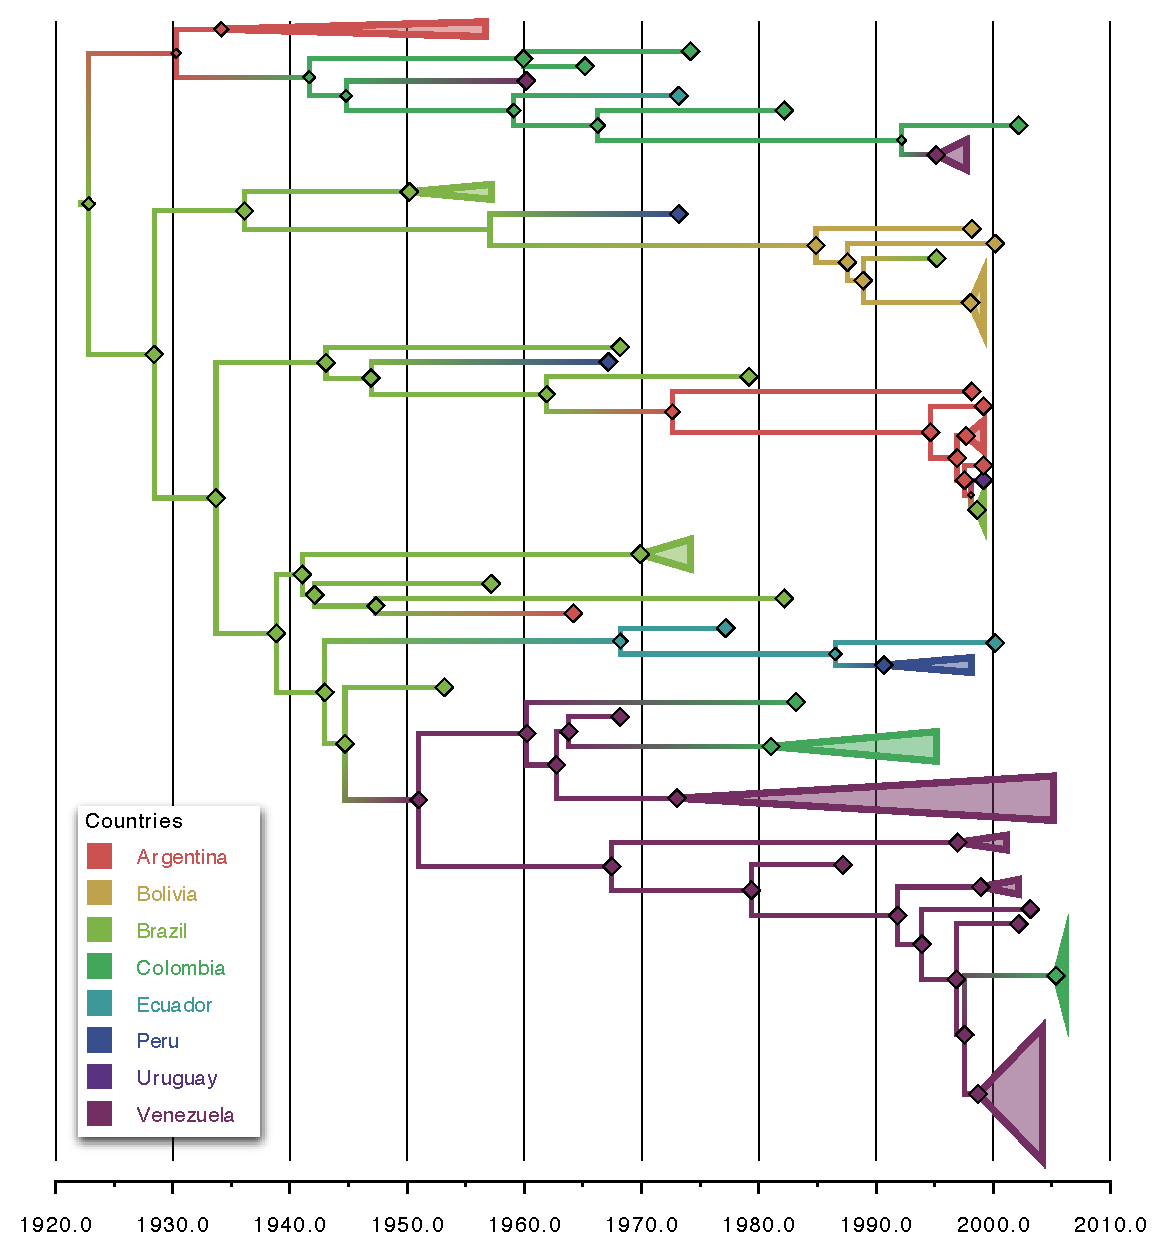
\includegraphics[scale=.45]{FIGURES/A.pdf}}\\
\subfigure[O]{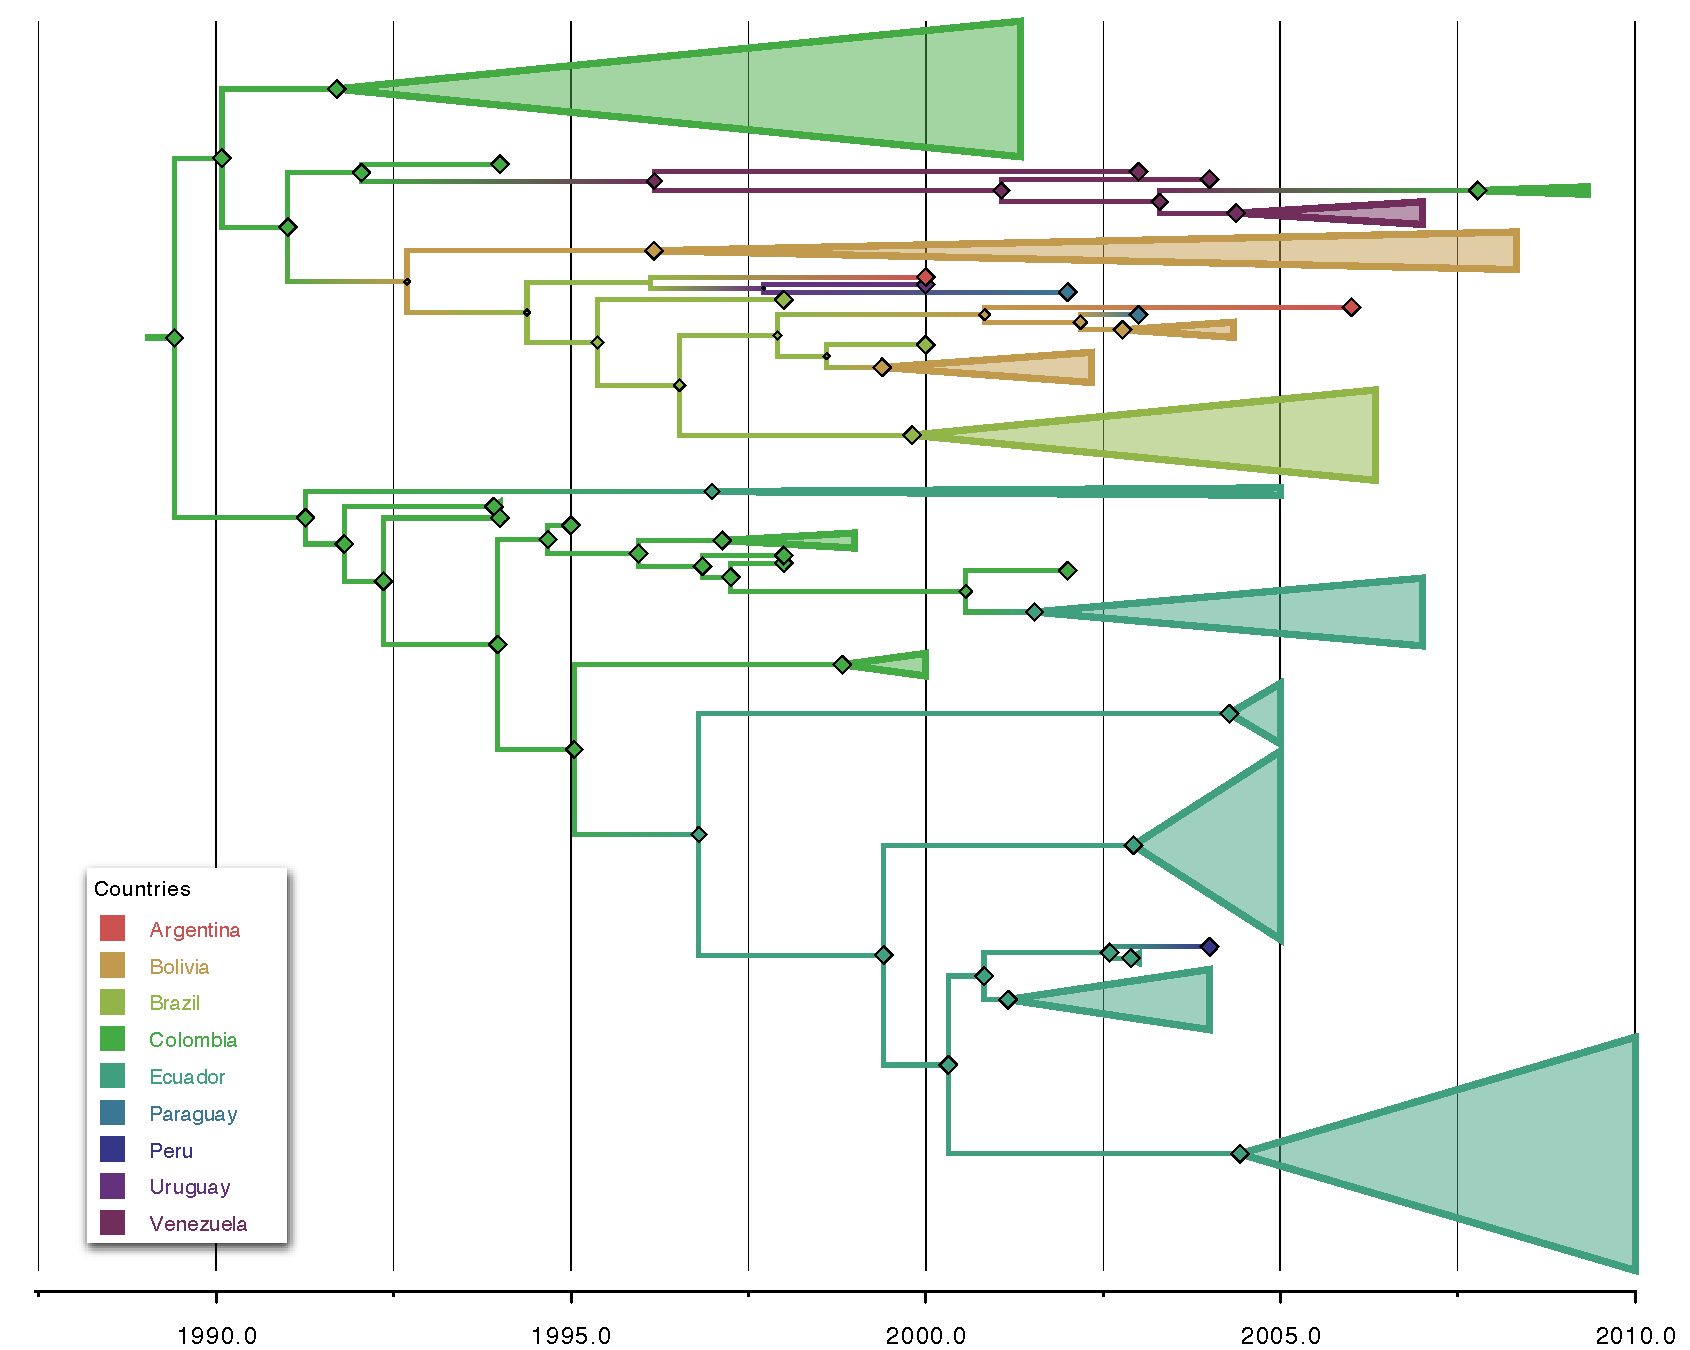
\includegraphics[scale=.30]{FIGURES/O.pdf}}
\end{center}
\caption{}
\label{fig:trees}
\end{figure}
%%%%%%%%%%%%%%%%%%%%%%%%%%
%%%%%%%%%%%%%%%%%%%%%%%%%%
\newpage
\begin{figure}[H]
\begin{center}
\subfigure[A --1945 ]{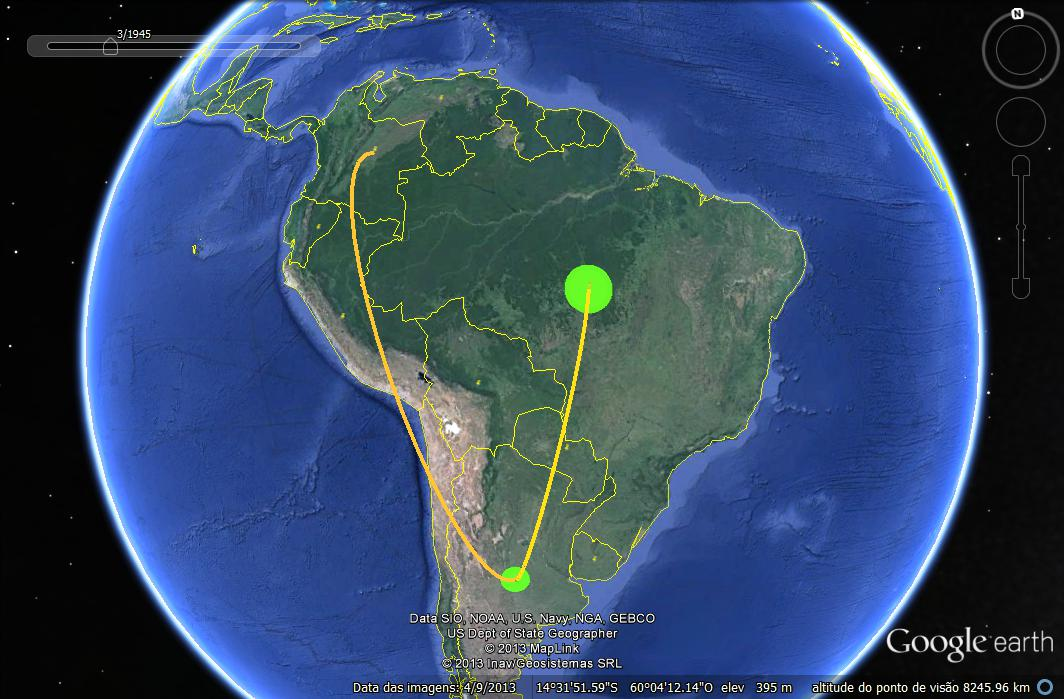
\includegraphics[scale=.20]{FIGURES/A_1945.jpg}}
\subfigure[O --1995 ]{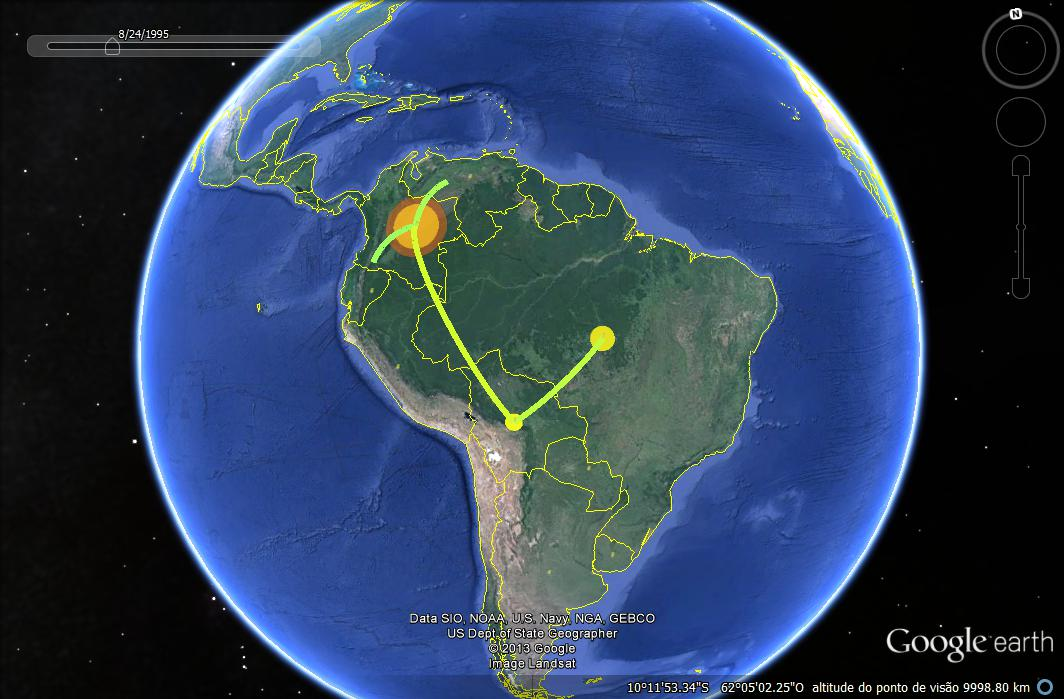
\includegraphics[scale=.20]{FIGURES/O_1995.jpg}}\\
\subfigure[A --1965 ]{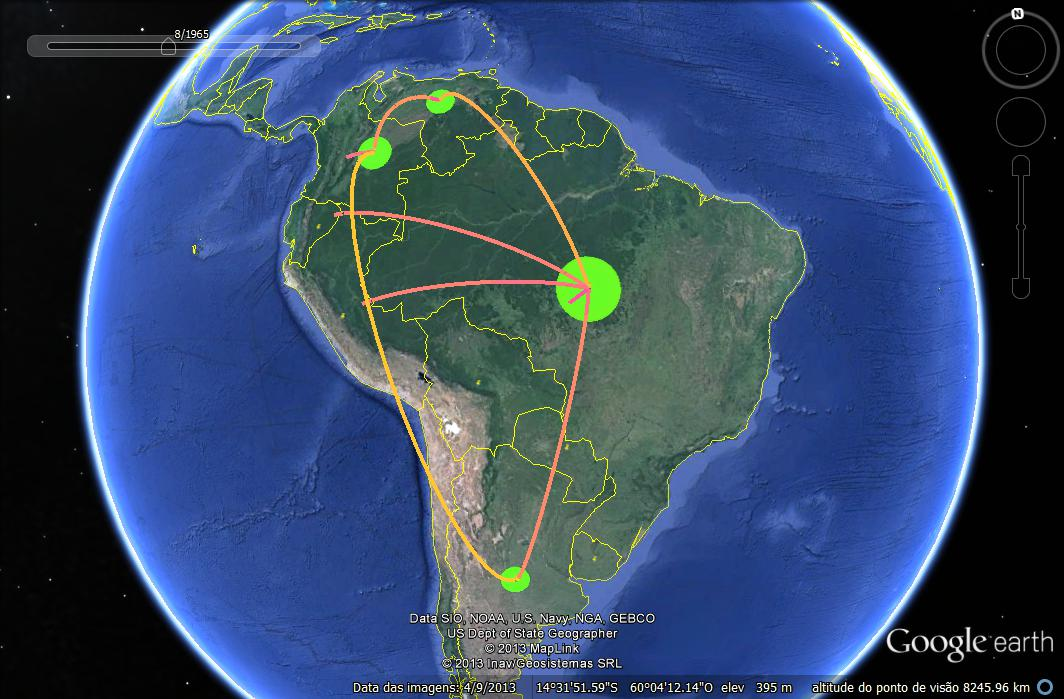
\includegraphics[scale=.20]{FIGURES/A_1965.jpg}}
\subfigure[O --2000 ]{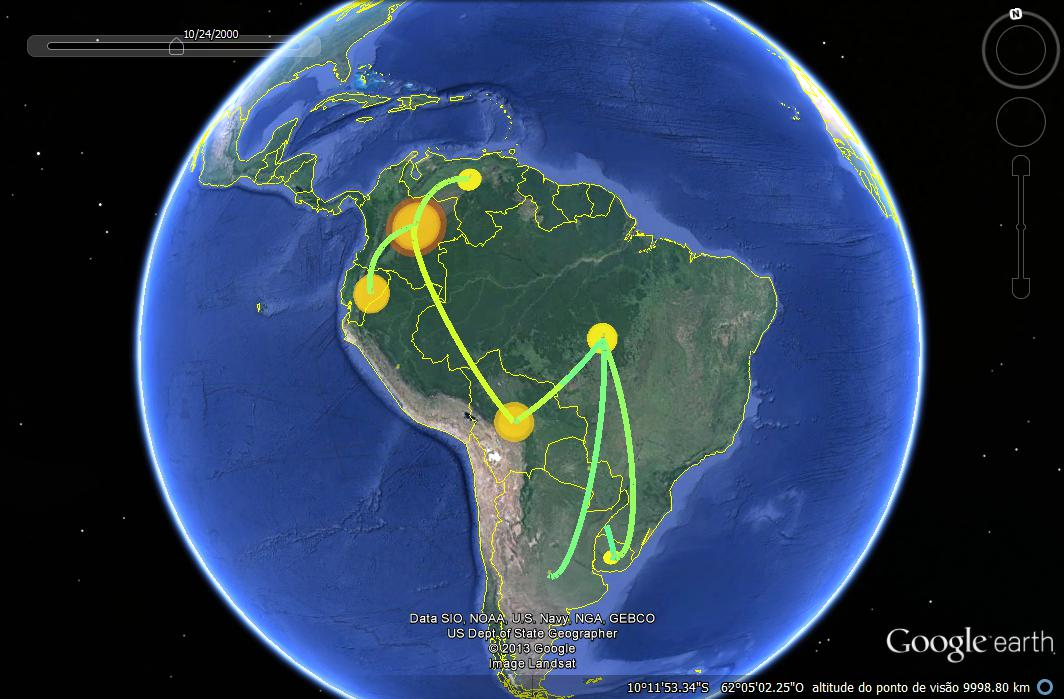
\includegraphics[scale=.20]{FIGURES/O_2000.jpg}}\\
\subfigure[A --1980 ]{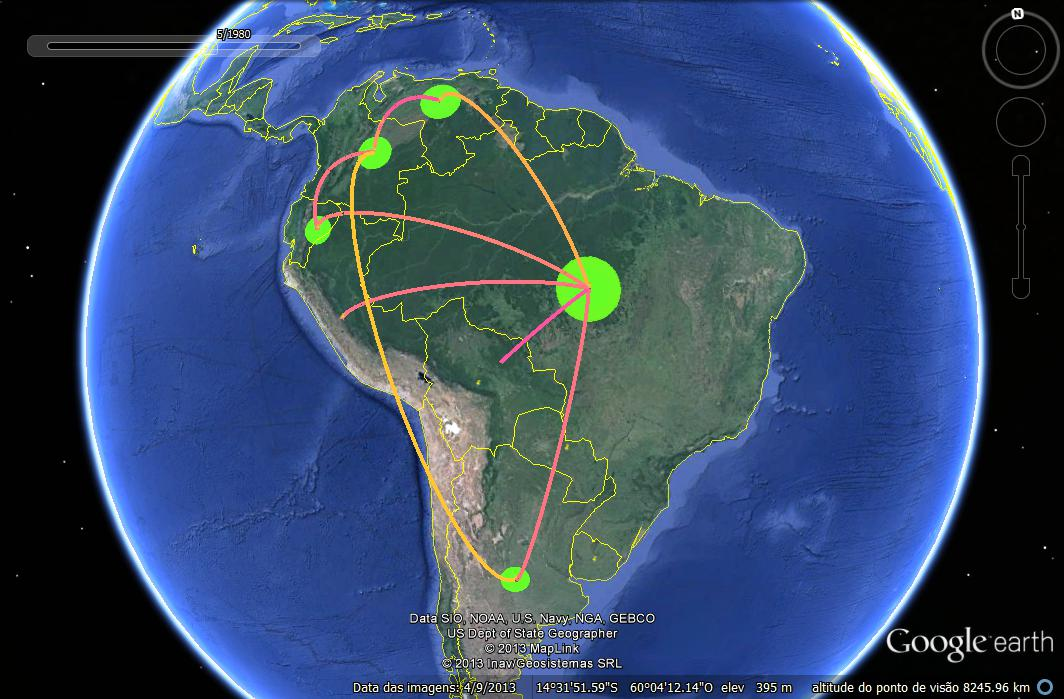
\includegraphics[scale=.20]{FIGURES/A_1980.jpg}}
\subfigure[O --2005 ]{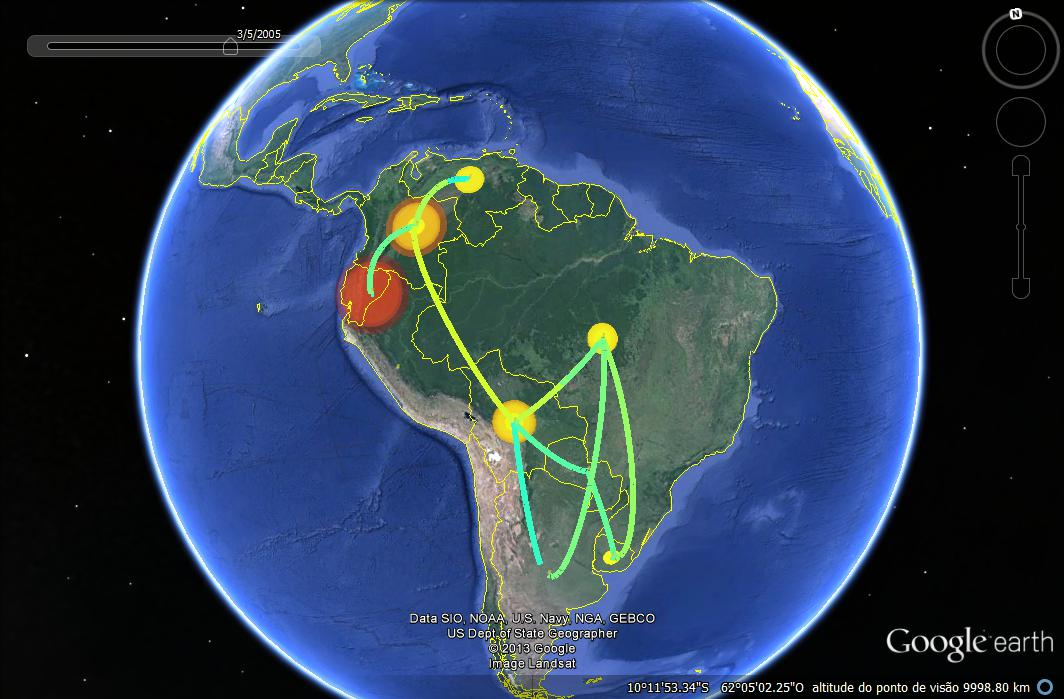
\includegraphics[scale=.20]{FIGURES/O_2005.jpg}}\\
\subfigure[A --2008 ]{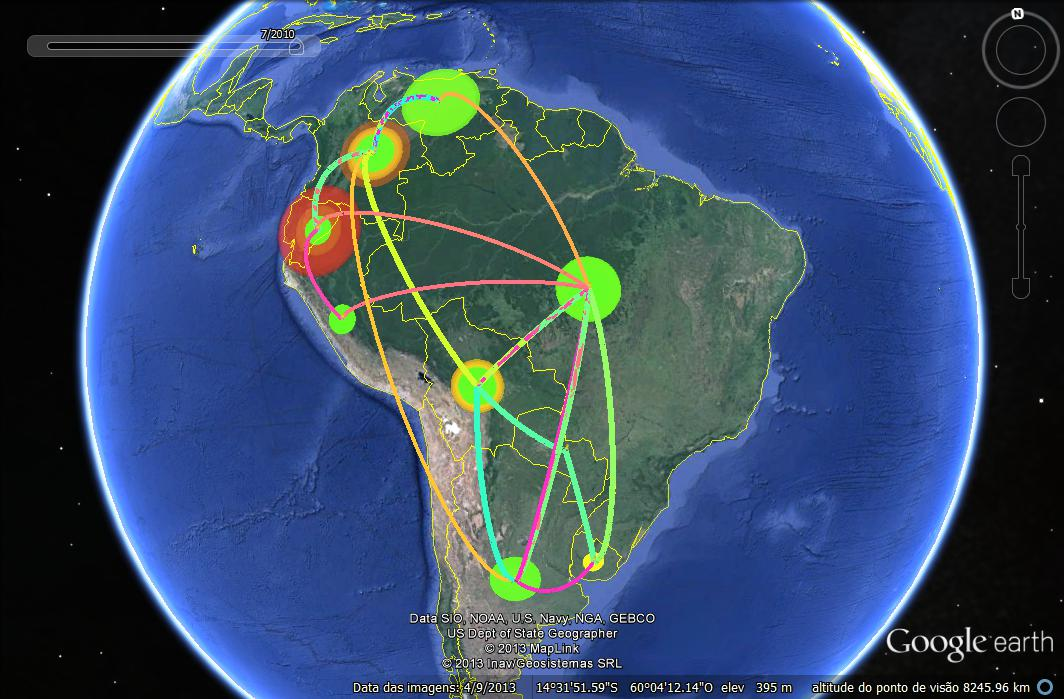
\includegraphics[scale=.20]{FIGURES/A_2008.jpg}}
\subfigure[O --2010 ]{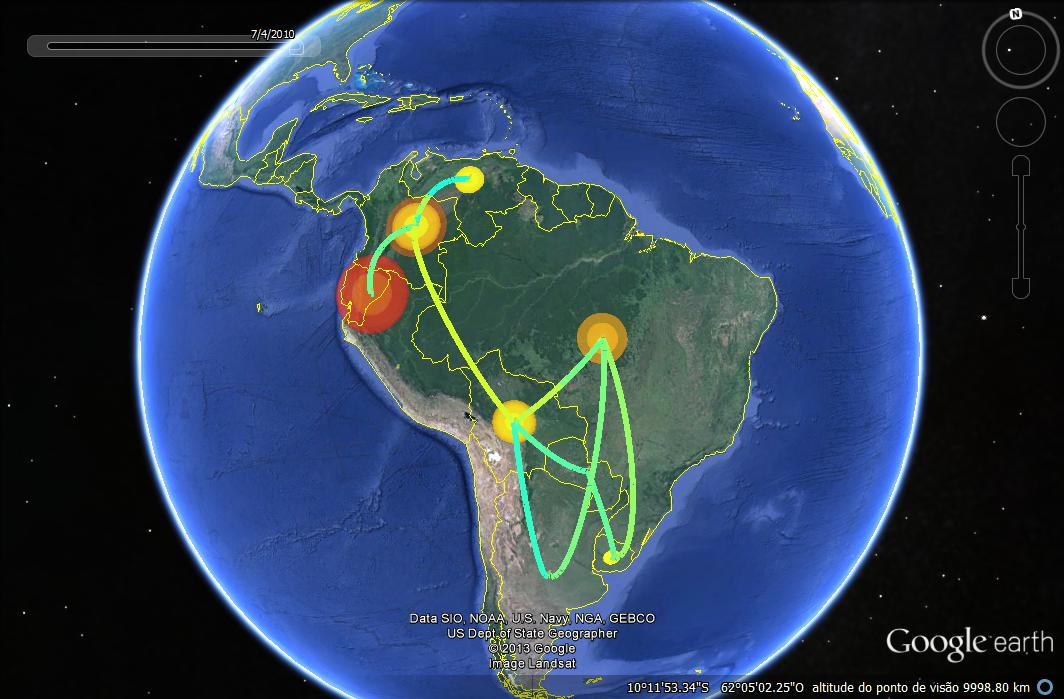
\includegraphics[scale=.20]{FIGURES/O_2010.jpg}}
\end{center}
\caption{}
\label{fig:migration}
\end{figure}
%%%%%%%%%%%%%%%%%%%%%%%%%%
%%%%%%%%%%%%%%%%%%%%%%%%%%
\newpage
\begin{figure}[H]
\begin{center}
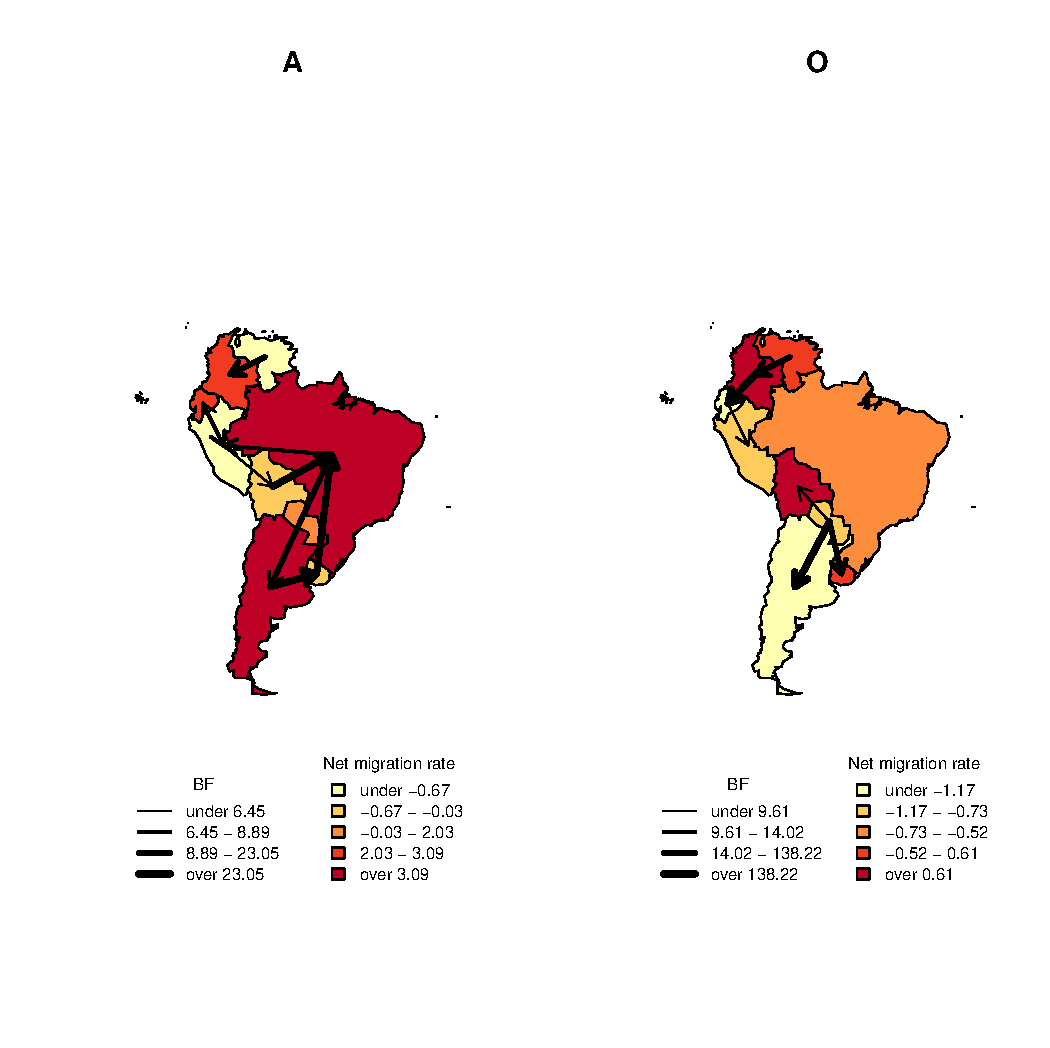
\includegraphics[scale=.85]{FIGURES/compound.pdf}
\end{center}
\caption{}
\label{fig:mj&BFs}
\end{figure}
%%%%%%%%%%%%%%%%%%%%%%%%%%
%%%%%%%%%%%%%%%%%%%%%%%%%%
\newpage
\begin{figure}[H]
\begin{center}
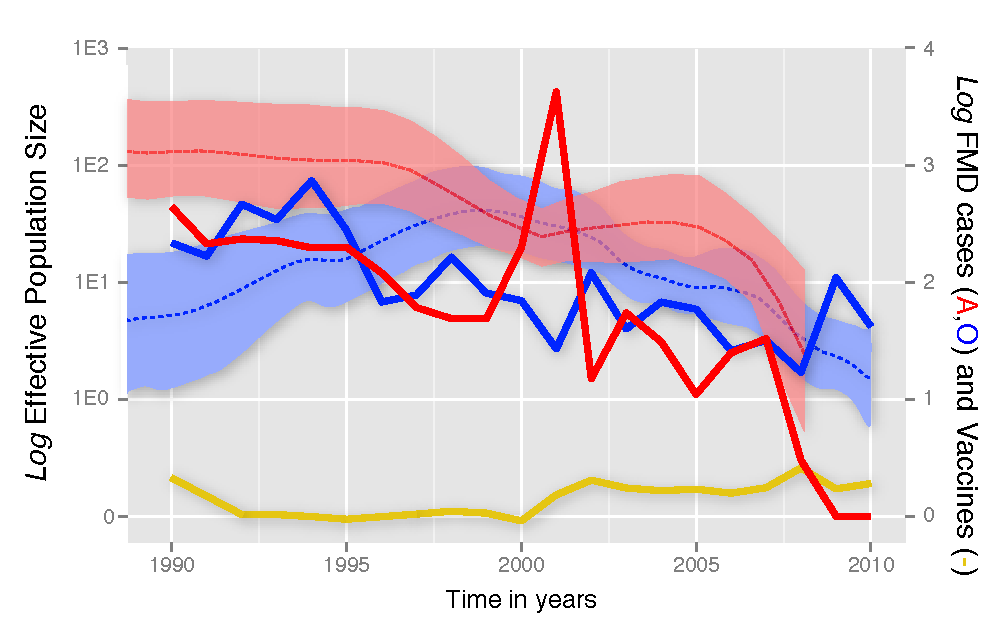
\includegraphics[scale=1.0]{FIGURES/skyride.pdf}
\end{center}
\caption{}
\label{fig:skyride}
\end{figure}
%%%%%%%%%%%%%%%%%%%%%%%%%%
%%%%%%%%%%%%%%%%%%%%%%%%%% 
\newpage
\begin{table}[H]
\caption{
\textbf{Spatial model selection results for epidemiological predictors.}
We assessed the significance of livestock trade in FMDV spread in South America using two importance sampling methods, path sampling (PS) and stepping-stone sampling (SS), to estimate (log) marginal likelihoods for each predictor using $64$ path steps and $2$ million iterations per path step, and corresponding Bayes factor (BF) comparisons.
We also present the (log) marginal likelihood estimates for two location priors under which the location rates are estimated, rather than being fixed (as for the livestock predictors).
%We put these two scenarios in a separate part of the table to indicate that these estimates should not be compared to those of the livestock predictors.
}
\begin{center}
\begin{tabular}{lrrrrrr}
\toprule
 & \multicolumn{3}{c}{Serotype A}& \multicolumn{3}{c}{Serotype O}\\
 \midrule
Predictor & PS & SS & log BF$^2$ & PS & SS & log BF \\
%\hline
Cattle&-12588.76&-12591.26&-27.70&\textbf{-8308.94}&\textbf{-8311.21}& \textbf{13.49}\\
Distance&\textbf{-12557.69}&\textbf{-12559.73}&\textbf{3.83}&-8313.89&-8315.37&9.33\\
Pigs&-12589.33&-12590.94&-27.38&-8325.39&-8326.63&-1.93\\
Sheep&-12570.67&-12572.56&-9.00&-8326.23&-8330.64&-5.94\\
Equal rates &-12561.98&-12563.56&--&-8321.49&-8324.70&--\\
\bottomrule
\end{tabular}
\end{center}
\begin{flushleft}
\end{flushleft}
\label{tab:preds}
 \end{table}
%%%%%%%%%%%%%%%%%%%%%%%%
%%%%%%%%%%%%%%%%%%%%%%%%
\newpage
\begin{table}[H]
\caption{
\textbf{Inferred root locations for each predictor for both serotypes.} We present most probable country of origin inferred using each predictor, with associated probabilities inside parentheses. 1-- all rates equal; 2-- Probability of being the root; 3-- Kullback-Leibler Divergence.
}
\begin{center}
\begin{tabular}{lcccc}
\toprule
& \multicolumn{2}{c}{Serotype A}&\multicolumn{2}{c}{Serotype O}\\
Predictor& Origin ($Pr$(root)$^2$)& KL$^3$&Origin ($Pr$(root))& KL\\
\midrule
Distance & Argentina ($0.75$)& $3.86$ & Colombia ($0.96$)& $3.76$\\
Sheep    & Brazil ($0.89$) & $3.52$ & Colombia ($0.99$)& $5.91$\\
Pigs      & Colombia ($0.99$)& $5.98$& Colombia ($0.91$)& $4.73$\\
Equal rates$^1$  & Argentina ($0.84$)& $3.78$ &Colombia  ($0.96$)& $3.20$\\
Cattle   & Peru ($0.93$)& $5.17$ & Colombia ($0.95$)& $3.81$\\
 \bottomrule
\end{tabular}
\end{center}
\begin{flushleft}
\end{flushleft}
\label{tab:roots}
 \end{table}
%%%%%%%%%%%%%%%%%%%%%%%%
\end{document}